\icode{N17J-MM-CA-L3-261012-001}
\nceeID[16]{2017天津}{12}
如图所示，物块\(A\)和\(B\)通过一根轻质不可伸长的细绳连接，跨放在质量不计的光滑定滑轮两侧，质量分别为\(m_A =\) \,\qty{2}{kg}、\(m_B =\)\,\qty{1}{kg}。初始时\(A\)静止与水平地面上，\(B\)悬于空中。先将\(B\)竖直向上再举高\(h =\)\,\qty{1.8}{m}（未触及滑轮）然后由静止释放。一段时间后细绳绷直，\(A\)、\(B\)以大小相等的速度一起运动，之后\(B\)恰好可以和地面接触。取\(g =\)\,\qty{10}{m/s^2}。
\begin{enumerate}
	\item \(B\)从释放到细绳绷直时的运动时间\(t\)；
	\item \(A\)的最大速度\(v\)的大小；
	\item \(B\)离地面的高度\(H\)。
\end{enumerate}
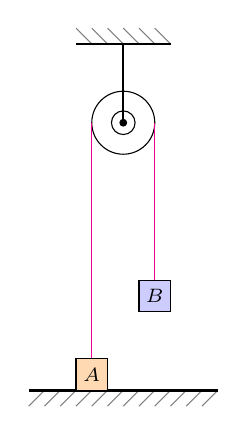
\begin{tikzpicture}[font=\scriptsize]
	\foreach \x in {-1.2,-1,...,1}
		\draw[gray] (\x,-3.6)--++(.2,.2);
	\foreach \x in {-.6,-.4,...,.6}
		\draw[gray] (\x,1.2)--++(.2,-.2);
	\draw[thick] (-1.2,-3.4)--(1.2,-3.4) (-.6,1)--(.6,1) (0,0)--(0,1);
	\draw (0,0) circle(.4) (0,0) circle(.15);
	\fill (0,0) circle(.05);
	\draw[magenta] (-.4,0)--(-.4,-3) (.4,0)--(.4,-2);
	\draw[fill=orange!30] (-.6,-3) rectangle(-.2,-3.4)node[pos=.5]{\(A\)};
	\draw[fill=blue!20] (.6,-2) rectangle(.2,-2.4)node[midway]{\(B\)};
\end{tikzpicture}
\begin{answer}
   （1）\(t =\) \qty{0.6}{s}（2）\(v =\) \qty{2}{m/s}（3）\(H =\) \qty{0.6}{m}\qquad 提示：绳子绷紧相当于完全非弹性碰撞；\(B\)恰好可以与地面接触，即\(B\)接地时速度为0
\end{answer}